\chapter{\'Etat de l'art}
	\section{Théorie des arbres d'attaque et de défense}
		Le concept des arbres d'attaques a été créé en 1999 par Bruce Schneier, un expert américain en securité informatique qui est parti du constat que des systèmes réputés "inviolables" se font briser en permance. De plus, ces systèmes sont brisés non pas en passant au travers des défenses mises en place, mais par des méthodes d'accès qui n'avaient pas été imaginées par ses concepteurs, car ils n'avaient pas les outils pour dresser une liste exhaustive des manières d'attaquer leur système. Il a donc créé le concept des arbres d'attaque dans ce but : pouvoir réaliser un inventaire exhaustif des méthodes d'attaque sur un système, quel qu'il soit, afin de pouvoir en concevoir la défense de la manière la plus complète possible.

		Lors de ces recherches, Mr Schneier a retenu un formalisme prècis : Une représentation des menaces sous la forme d'arbres. Ces arbres sont réalisés en se posant la question suivant : Si je veux atteindre tel objectif, qu'est ce que cela pré-suppose que j'accomplisse d'abord ? Pour cela, on représente l'objectif final en haut de l'arbre, et l'on ajoute en descendant dans l'arbre les objectifs intermédiaires (noeuds) plus simples à réaliser, qui nous garantissent l'accomplissement de l'objectif principal. L'on fait ensuite découler de ces objectifs intermédiaires d'autres objectifs les validant, etc... jusqu'à avoir en bas de l'arbre des actions simples (feuilles). Ensuite, il suffit de descendre dans l'arbre à partir d'un noeud pour savoir quelles sont les combinaisons d'actions possibles à effectuer pour atteindre le noeud. 

		L'arbre de la figure \ref{fig:arbre_exemple_1} illustre ce formalisme : 

		\begin{figure}
			\begin{center}
				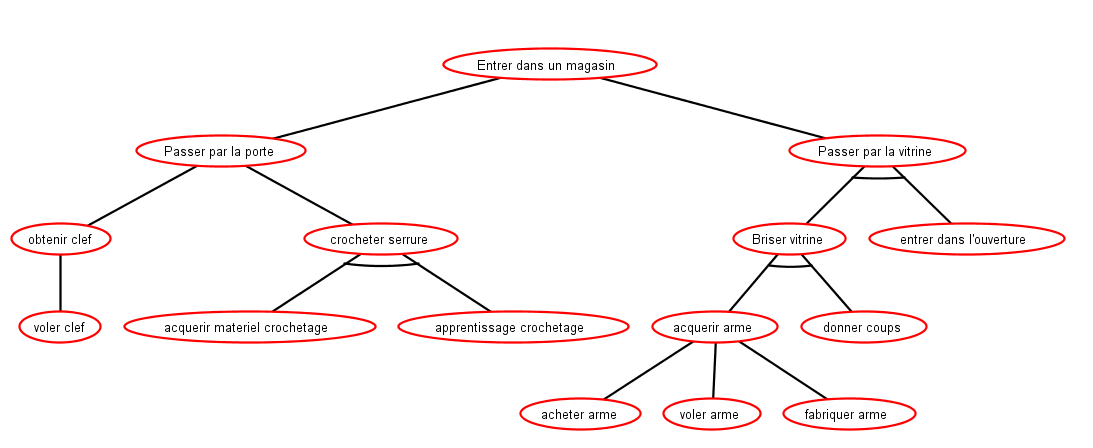
\includegraphics[width=0.8\textwidth]{figure/Entrer_dans_un_magasin.png}
			\end{center}
			\caption{C'est tres bien}
			\label{fig:arbre_exemple_1}
		\end{figure}

		Aussi, le concept original de Schneier intègre la possibilté d'associer aux feuilles des valeurs représentatives de diverses informations sur l'accomplissement de l'action : coût, difficulté, probabilité, temps d'exécution, etc... Il est alors possible à partir de ces valeurs de pouvoir quantifier ces mêmes informations pour les noeuds qui en découlent.

		Depuis 1999, le concept a évolué grâce à la contribution de personnes ayant étendu et amélioré le concept de Mr Schneier : Barbara Kordy, Sjouke Mauw, Saša Radomirović, Patrick Schweitzer. Ces personnes ont en pareticulier étendu le concept d'arbre d'attaque à celui d'arbre de défense, où sont également reprséntés les defenses mises en place et que le potentiel attaquant aura besoin de désactiver pour atteindre son but. Un formalisme existe aussi pour ces types d'arbres ADT (Attack Defense Tree), où les défense sont représentées dans des rectangles et liés avec des pointillés. Le même arbre que précédemment avec des défenses ressemble à la figure \ref{fig:arbre_exemple_2}.

		\begin{figure}
            \begin{center}
                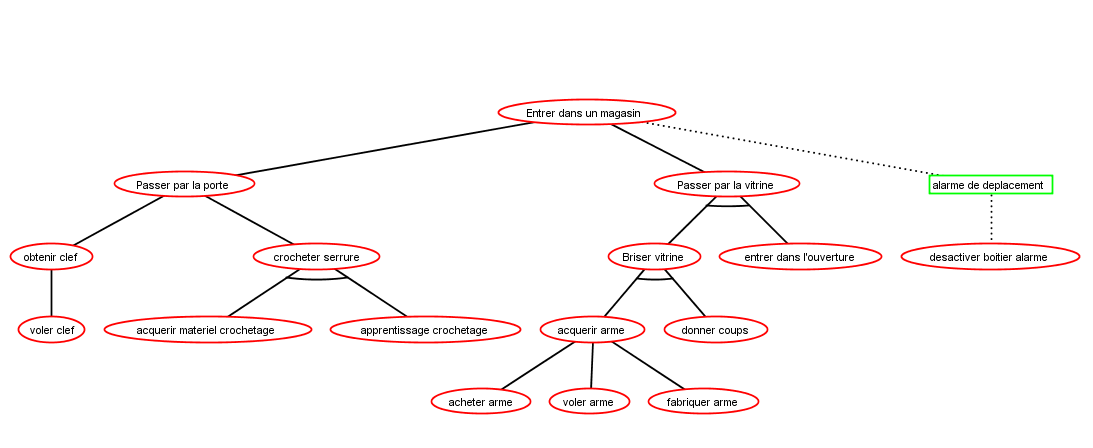
\includegraphics[width=0.8\textwidth]{figure/Entrer_dans_un_magasin2.png}
            \end{center}
            \caption{Entrer dans la magasin 2.}
            \label{fig:arbre_exemple_2}
		\end{figure}

	\section{Implémentations des ADT}
		Plusieurs logiciels implémentant le concept des ADT ont été développés. Voici les principaux :
		\large Logiciels propriétaires :
		\begin{itemize}
			\item SecurlTree
			\item ATTACKTREE+
		\end{itemize}
		~~\\
		\large Logiciels Open-Source :
		\begin{itemize}
			\item ADTool
		\end{itemize}

		\iffalse{}
		Biblio :
		https://www.schneier.com/paper-attacktrees-ddj-ft.html
		http://www.sciencedirect.com/science/article/pii/S1574013714000100
		http://logcom.oxfordjournals.org/content/24/1/55
		\fi